\section{Durchführung}
\begin{figure}[tb]
  \centering
  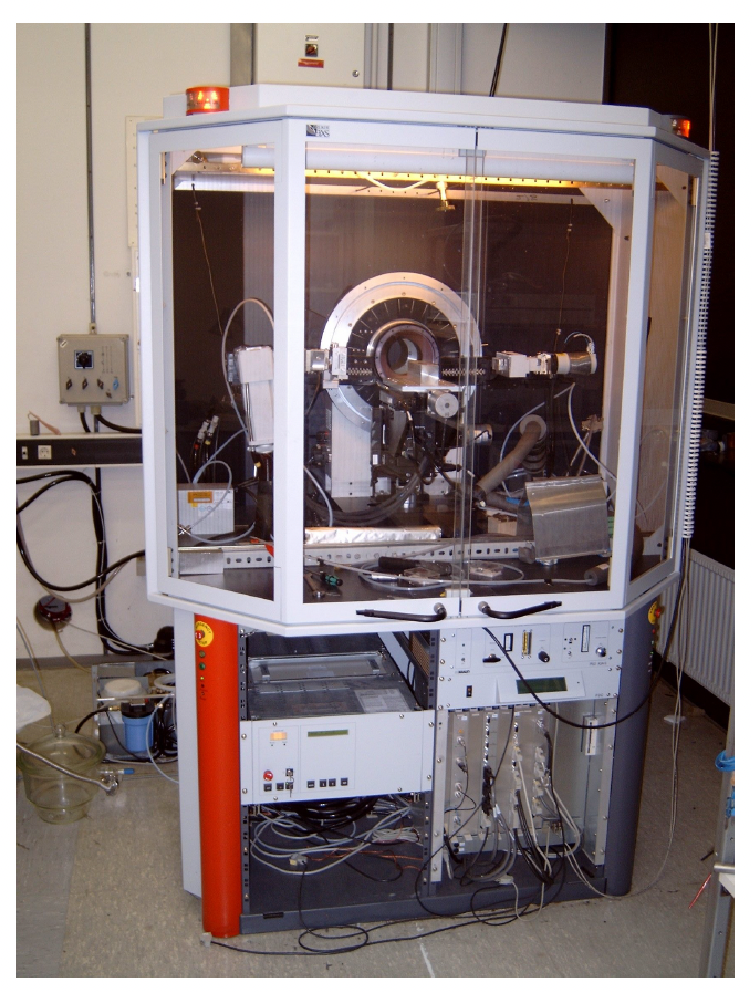
\includegraphics[width=8cm,keepaspectratio]{diffraktometer.png}
  \caption{Das verwendete D8-Labordiffraktometer der Firma Bruker-AXS.}
  \label{fig:diffrac}
\end{figure}
Die Durchführung lässt sich grob in zwei Teile gliedern: zunächst wird die Justage des Versuchsaufbaus erläutert und im Weiteren die eigentliche Messreihe.

Für die Versuchsdurchführung wird das D8-Labordiffraktometer der Firma Bruker-AXS verwendet, wie es in \autoref{fig:diffrac} zu sehen ist. Dieses beinhaltet den Probentisch, sowie eine Röntgenröhre und einen Detektor, die um den Probentisch drehbar sind. Zur Bedienung der Apparatur und der Aufnahme der Messwerte wird das Programm \textit{XRD Commander} verwendet. Die erhaltenen Messdaten werden im .raw-Format abgespeichert und für die Auswertung mit dem Programm \textit{File Exchange} in .uxd-Dateien umgewandelt. Vor Beginn der ersten Messung muss der maximale Absorber eingeschaltet werden, damit Schäden am Detektor vermieden werden.

\subsection{Justage}
\begin{table}[tb]
  \centering
  \caption{Angaben zu Messbereich und -Intervall für die einzelnen Justage-Scans.}
  \begin{tabular}{l c c c}
    \toprule
    Typ & Messbereich/° & Schrittweite/° & Messdauer pro Messpunkt/s \\
    \midrule
    Detektorscan & $\num{-0.5}$ bis $\num{0.5}$ & $\num{0.02}$ & $1$ \\
    Z-Scan & $\num{-1}$ bis $\num{1}$ & $\num{0.04}$ & $1$ \\
    Rockingscan $2\theta = 0$ & $\num{-1}$ bis $\num{1}$ & $\num{0.04}$ & $1$ \\
    Z-Scan & $\num{-0.5}$ bis $\num{0.5}$ & $\num{0.02}$ & $1$ \\
    Rockingscan $2\theta = \num{0.3}$ & $\num{0}$ bis $\num{0.3}$ & $\num{0.005}$ & $1$ \\
    Z-Scan $2\theta = \num{0.3}$ & $\num{-0.5}$ bis $\num{0.5}$ & $\num{0.02}$ & $1$ \\
    \bottomrule
  \end{tabular}
  \label{tab:justage}
\end{table}

Messbereiche und weitere Informationen zu den einzelnen Justage-Scans sind \autoref{tab:justage} zu entnehmen.
Die Justage wird begonnen mit einem Detektorscan.
Hierfür wird der Probentisch aus dem Strahlengang gefahren. Der Scan dient dazu, die $\SI{0}{\degree}$-Lage des Detektors zu bestimmen.
Ist diese ermittelt und gespeichert worden, wird ein erster Z-Scan durchgeführt. Dieser ermittelt die Position des Strahls, sodass die Probe die halbe Strahlintensität abdeckt.
Da der Z-Scan nicht sensitiv auf die parallele Ausrichtung des Strahls zur Probenoberfläche ist, wird daraufhin ein Rockingscan durchgeführt. Dieser entspricht einer Drehung der Probe im Strahlengang.
Da die Anpassung der Neigung auch die Abschattung ändert, wird im Anschluss ein zweiter Z-Scan gefahren, um wieder die Position halber Abschattung zu finden.
Zur noch exakteren Bestimmung der idealen Position werden daraufhin ein weiterer Rocking- und Z-Scan gefahren, diesmal unter einem Ein- und Ausfallswinkel von $\SI{0.15}{\degree}$.
Anschließend ist die Probe justiert.

\subsection{Messung eines Polymerfilmes auf einem Silizium-Wafer}
Der Messvorgang eines Polymerfilmes auf einem Silizium-Wafer besteht aus zwei Schritten. Zunächst wird ein Scan gefahren, bei dem der Einfallswinkel der Strahlung auf die Probe gleich dem Winkel zwischen Probe und Detektor ist. Hierbei wird ein Bereich von $\SIrange{0}{2.5}{\degree}$ abgefahren bei einer Schrittweite von $\SI{0.005}{\degree}$ und einer Messdauer pro Messpunkt von $\SI{5}{\second}$.

Zur Ermittlung der wahren Reflektivität wird daraufhin ein zweiter Scan mit den gleichen Einstellungen gefahren. Dieses Mal wird der Detektorwinkel allerdings so eingestellt, dass er $\SI{0.1}{\degree}$ gegenüber dem Einfallswinkel verschoben ist. So lässt sich der Anteil der gestreuten Intensität an der Reflektivität bestimmen, welcher dann von der ersten Messreihe abgezogen wird.
